\chapter{Data integration: a data representation-independent approach}\label{cha:dataintegration}

\epigraph{\textit{
		Logic is the most useful tool of all the arts. Without it no science can be fully known. It is not worn out by repeated use, after the manner of material tools, but rather admits of continual growth through the diligent exercise of any other science. For just as a mechanic who lacks a complete knowledge of his tool gains a fuller [knowledge] by using it, so one who is educated in the firm principles of logic, while he painstakingly devotes his labor to the other sciences, acquires at the same time a greater skill at this art.
	}}{--- William of Ockham, \textit{Summa Logic\ae}, Prefatory Letter}

\textbf{Data Integration} is a sequence of transformations (and hence, queries) through which all the data coming from different data sources are mapped (\textbf{transcoded}) to a \textit{reconciled representation} over a many-to-one data association (\textbf{alignment}). Each resulting value-representation (type) may be indistinguishable from the representation available from the data sources (uniform representation).

Data integration theory uses abstraction to generalise all the possible approaches which are data structure specific. Such theory focuses on the main preprocessing steps which are alignment and transcoding as introduced in the incoming introductory examples (Section \ref{sec:oldschooldi}). While languages and models outlining data representation abstraction were defined decades ago and date back to the studies on programming languages \cite{omg96,TPLPierce}, the theoretical approaches abstracting data integration process are more recent \cite{Lenzerini02,DeGiacomo2018}. This lack of formalisation made all the researcher focus more on the data integration aspect that are representation-dependent (\textit{how shall we integrate data with different ``shapes''}) than on the actual integration process (\textit{what makes data from different sources ``hard'' to integrate, independently from their representation?}). The latter takes stock of two different integrations (or fusion\footnote{In current literature, the term ``fusion'' assumes an ambiguous connotation: while anglophone literature \cite{Hall97,KHALEGHI201328} focuses on the integration of sensor unstructured data possibly with structured data (e.g. geospatial information), germanophone literature \cite{deII,Bleiholder09} calls ``data fusion'' (\textit{Datenfusion}) the process of data cleaning and conflict resolution that could be carried out within one same data source. This terminological ambiguity reveals two different aspects of performing data integration.}) which are ``In-Database integration'' (Section \ref{sec:informationsintegration}) and ``Multi-database integration'' (Section \ref{sec:integsurvey}). These specific topics allow to draw the following observations for both current query languages and data structures:
\begin{itemize}
\item  \textit{In-Database Integration} requires that joins and group by operations are generalised to the nesting operator, which enables structural aggregations (Section \ref{sec:informationsintegration}). Structural aggregations should allow representing data at different abstraction levels, where summarised and coarser representations coexist (Example \vref{ex:inaggr}). Current query languages and data structures do not meet these requirements.
\item \textit{Multi-database integration} requires that a query language should support all the operators used on different data representations (Section \ref{subsec:queryrw}) alongside with transcoding (Section \ref{sec:ontology}). Data representation should be able to represent data and alignments uniformly.
\end{itemize}


\begin{figure}[pt]
\begin{minipage}[t]{\textwidth}
  \centering
  \begin{minipage}[t]{\textwidth}
    \resizebox{\textwidth}{!}{%
    \begin{tabular}{llccccl}
      \toprule
      \textbf{SocialSecurityNo} &  \textbf{diagnosis} &  \textbf{week} &  \textbf{month} & \textbf{year} &  \textbf{ward} &  \textbf{ICD-9-CM} \cr
        \midrule
      BCDVHZ59S23F743S & Right parotid neoplastic formation & 1 & 1 & 2017 & Oncology &  210.2\\
      PNPMZZ74H45H782P & Relapsing epistaxis & 2 & 1 & 2017 & Emergency &  784.7\\
      PKTBMF36E14H842O & Septal deviation and nasal-sinus polyps & 3 & 1 & 2017 & Emergency & 748.1, 471.0\\
      \bottomrule
    \end{tabular}}
    \subcaption{\texttt{Admissions} table from the internal Data Warehouse.}
    \label{tab:Admissions}
  \end{minipage}

  \begin{minipage}[t]{\textwidth}
    \resizebox{\textwidth}{!}{%
    \begin{tabular}{lllcccl}
      \toprule
      \textbf{SocialSecurityNo} & \textbf{organ} & \textbf{disease} & \textbf{day} & \textbf{month} & \textbf{year} & \textbf{ward} \cr
        \midrule
      BCDVHZ59S23F743S & \texttt{NULL} & Right vestibular deficit & 2 & 1 & 2017 & Emergency\cr % 386.10
      PNPMZZ74H45H782P & Appendix & Severe Appendicitis & 17 & 2 & 2017 & Emergency\cr % 540.9
      PKTBMF36E14H842O & Intestine & Recanalization of Crohn's Disease & 25 & 3 & 2017 & Emergency\cr % 555.0
      \bottomrule
    \end{tabular}}
    \subcaption{\texttt{Hospitalization} table from an external Data Warehouse.}
    \label{tab:Hospitalization}
  \end{minipage}

  \begin{minipage}[t]{\textwidth}
    \resizebox{\textwidth}{!}{%
    \begin{tabular}{llccccl}
      \toprule
      \textbf{SocialSecurityNo} &  \textbf{diagnosis} &  \textbf{week} &  \textbf{month} & \textbf{year} &  \textbf{ward} &  \textbf{ICD-9-CM} \cr
        \midrule
      BCDVHZ59S23F743S & Right parotid neoplastic formation & 1 & 1 & 2017 & Oncology &  210.2\\
      BCDVHZ59S23F743S & Right vestibular deficit & 2 & 1 & 2017 & Emergency & 386.10\cr
      PNPMZZ74H45H782P & Relapsing epistaxis & 2 & 1 & 2017 & Emergency &  784.7\\
      PNPMZZ74H45H782P & Severe Appendicitis & 8 & 2 & 2017 & Emergency & 540.9\cr %
      PKTBMF36E14H842O & Septal deviation and nasal-sinus polyps & 3 & 1 & 2017 & Emergency & 748.1, 471.0\\
      PKTBMF36E14H842O & Recanalization of Crohn's Disease & 15 & 3 & 2017 & Emergency & 555.0\cr %
      \bottomrule
    \end{tabular}}
    \subcaption{Expected result for the integration of the two upper tables.}
    \label{tab:MergedTables}
  \end{minipage}

  \caption{Integrating two tables (\subref{tab:Admissions} and \subref{tab:Hospitalization}) pertaining to hospitalization into one final table (\subref{tab:MergedTables}), matching with the schema of \subref{tab:Hospitalization}. Diagnoses and diseases were obtained from the ``ICD code it'' dataset, available at \url{smartdata.cs.unibo.it}, while the other parts are randomly generated.\hrule}
  \label{fig:examplesrelational}
\end{minipage}
% ---- %%%%%%%
\begin{minipage}[t]{\textwidth}
	\vspace*{1cm}
  \begin{minipage}[t]{\textwidth}
    \centering
    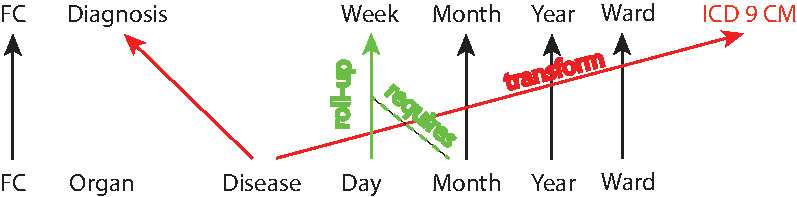
\includegraphics[width=.8\textwidth]{fig/01dataint/AlignmentRelational01.pdf}
    \subcaption{Alignment between the schemas of the two data sources. Data types associated to each field are not showed.}
    \label{fig:relalign}
  \end{minipage}

    \begin{minipage}[t]{\textwidth}
      \resizebox{\textwidth}{!}{%
      \begin{tabular}{lllcccl}
        \toprule
        \textbf{SocialSecurityNo} & \textbf{disease} & \textbf{week} & \textbf{month} & \textbf{year} & \textbf{ward} & \textbf{ICD-9-CM} \cr
          \midrule
        BCDVHZ59S23F743S & Right vestibular deficit & $\stigma(2,1)$ & 1 & 2017 & Emergency & $\stigma'($Rigth\dots $)$\cr % 386.10
        PNPMZZ74H45H782P & Severe Appendicitis & $\stigma(17,2)$ & 2 & 2017 & Emergency & $\stigma'($Severe\dots $)$\cr % 540.9
        PKTBMF36E14H842O & Recanalization of Crohn's Disease & $\stigma(25,1)$ & 3 & 2017 & Emergency & $\stigma'($Recanalization\dots $)$\cr % 555.0
        \bottomrule
      \end{tabular}}
      \subcaption{Record transformation for \texttt{Hospitalization} after the alignment with \texttt{Admissions}.}
      \label{tab:HospitalizationAlign}
    \end{minipage}

    \begin{minipage}[t]{\textwidth}
      \resizebox{\textwidth}{!}{%
      \begin{tabular}{lllcccl}
        \toprule
        \textbf{SocialSecurityNo} & \textbf{disease} & \textbf{week} & \textbf{month} & \textbf{year} & \textbf{ward} & \textbf{ICD-9-CM} \cr
          \midrule
        BCDVHZ59S23F743S & Right vestibular deficit & 2 & 1 & 2017 & Emergency & 386.10\cr %
        PNPMZZ74H45H782P & Severe Appendicitis & 8 & 2 & 2017 & Emergency & 540.9\cr %
        PKTBMF36E14H842O & Recanalization of Crohn's Disease & 15 & 3 & 2017 & Emergency & 555.0\cr %
        \bottomrule
      \end{tabular}}
      \subcaption{Resolution of the  transcoding functions $\stigma$ over the aligned \texttt{Hospitalization}}
      \label{tab:HospitalizationTransf}
    \end{minipage}

    \caption{Data integration steps: intermediate schema alignment and transcoding transformation steps before providing the final result.}
\end{minipage}
\end{figure}
